% Chapter 1

\chapter{Introducción general} % Main chapter title

\label{Chapter1} % For referencing the chapter elsewhere, use \ref{Chapter1} 
\label{IntroGeneral}
En este capítulo se presentan los principales tipos de paneles de mensajes variables, las características de las pantallas full color y por último se explica el alcance y objetivos.
%----------------------------------------------------------------------------------------

% Define some commands to keep the formatting separated from the content 
\newcommand{\keyword}[1]{\textbf{#1}}
\newcommand{\tabhead}[1]{\textbf{#1}}
\newcommand{\code}[1]{\texttt{#1}}
\newcommand{\file}[1]{\texttt{\bfseries#1}}
\newcommand{\option}[1]{\texttt{\itshape#1}}
\newcommand{\grados}{$^{\circ}$}

%----------------------------------------------------------------------------------------

%\section{Introducción}

%----------------------------------------------------------------------------------------
\section{Pantallas de mensaje variable}

Los paneles de mensajes variables son señales de tránsito diseñadas para alertar o informar al usuario de la carretera. El panel de mensajes variable puede mostrar pictogramas o mensajes escritos, las imágenes en pantalla pueden ser estáticas, parpadeantes o realizar efectos\cite{WIKIVMS}.
%\agregar referencia bibl. 
%\https://es.wikipedia.org/wiki/Panel_de_mensajes_variables#cite_note-1

\subsection{Panel de mensajes variables fijo}

Los paneles de mensajes variables fijos generalmente se montan en estructuras aéreas que abarcan la carretera, en voladizo sobre una parte de la carretera, o fuera de la carretera, y se utilizan para influir en los automovilistas con propósitos de control de tránsito. Sus mensajes pueden cambiarse manual, mecánica o electro-mecánicamente para proporcionar a los automovilistas información sobre congestión del tráfico, accidentes de tráfico, operaciones de mantenimiento, condiciones climáticas adversas, condiciones de la carretera, eventos organizados u otras características de la carretera. Un beneficio de los paneles de mensajes variables permanentes es que pueden soportar un mayor tiempo, desplegar mensajes más detallados y permitir un mayor tiempo de exposición para que los automovilistas comprendan los mensajes antes de llegar a un punto de decisión.En la figura \ref{fig:vmsp} se muestra una pantalla de mensajes variables fijo\citep{VMSTYPES}.


\begin{figure}[htpb]
	\centering
	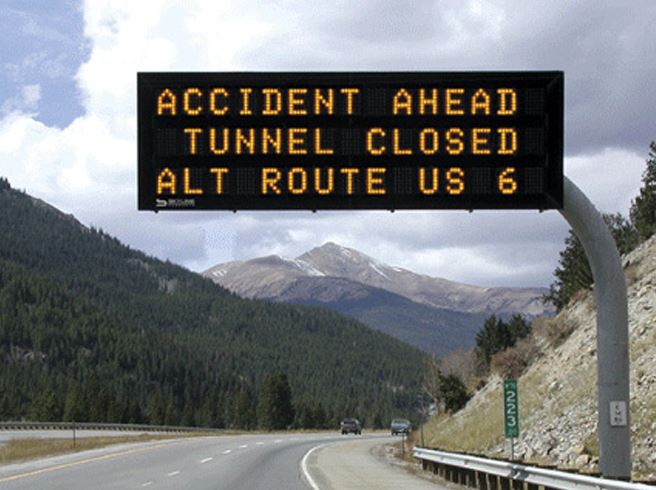
\includegraphics[width=.9 \textwidth]{../Figures/vmspermanente.jpg} 
	\caption{Panel de mensajes variables permanente \protect\footnotemark.}
	\label{fig:vmsp}
\end{figure}

\footnotetext{Imagen tomada de \url{https://www.skylineproducts.com/wp-content/uploads/2016/07/Walk-In.jpg}}


%----------------------------------------------------------------------------------------

%/ https://www.skylineproducts.com/wp-content/uploads/2016/07/Walk-In.jpg


\subsection{Panel de mensajes variables móvil}

Los paneles de mensajes variable móvil suelen estar montados en un remolque con paneles solares, son de fácil movimiento y pueden ser colocados cerca del punto de decisión. Sus mensajes se pueden cambiar de forma manual, mecánica o por medios electromecánicos para proporcionar a los automovilistas información sobre la congestión del tráfico, los accidentes de tráfico, operaciones de mantenimiento, condiciones climáticas adversas, condiciones de la carretera, eventos organizados u otros características de la carretera. Un beneficio de los paneles de mensajes variables móviles es la posibilidad de ubicación en puntos estratégicos.En la figura \ref{fig:vmsm} se muestra una pantalla de mensajes variables móvil\citep{VMSTYPES}.

\begin{figure}[htpb]
	\centering
	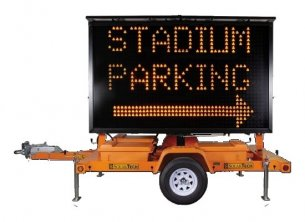
\includegraphics[width=.7\textwidth]{../Figures/vmsmovil.jpg} 
	\caption{Panel de mensajes variables móvil\protect\footnotemark.}
	\label{fig:vmsm}
\end{figure}
\footnotetext{Imagen tomada de \url{https://www.enterpriseflasher.com/assets/images/solartech-1364402479.jpg}}

%/ https://www.enterpriseflasher.com/assets/images/solartech-1364402479.jpg


\subsection{Panel de mensajes variables montado en camión}

Los Paneles de mensajes variables montados en camión son generalmente unidades pequeñas montadas en o cerca de la parte trasera de un camión. Los paneles montados en camión generalmente tienen espacio reducido para mensajes y tamaños de fuente. Las limitaciones de sus mensajes suelen resultar en el uso de gráficos como flechas para facilitar la comprensión del conductor\citep{VMSTYPES}.

\begin{figure}[htpb]
	\centering
	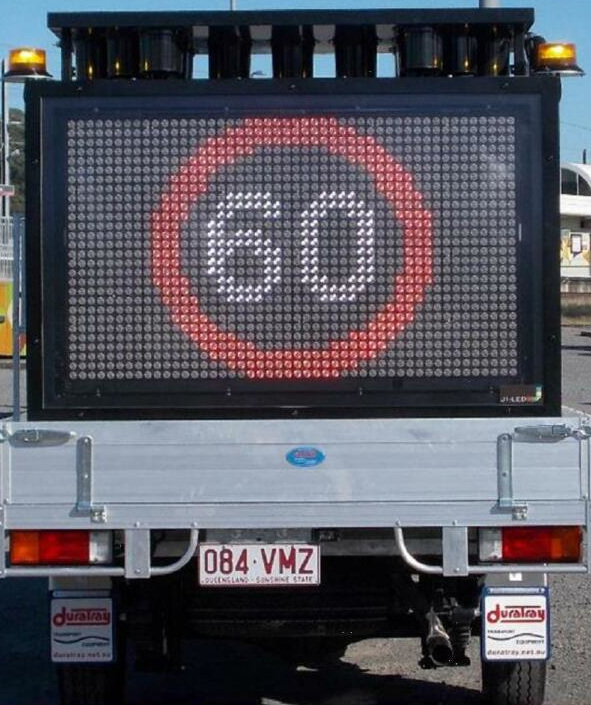
\includegraphics[scale=1]{../Figures/vmstruck.png} 
	\caption{Panel de mensajes variables montado en camión\protect\footnotemark.}
	\label{fig:vmsc}
\end{figure}
\footnotetext{Imagen tomada de  \url{https://www.mobilesystems.co.nz/vdb/image/i2123}}
%/ https://www.mobilesystems.co.nz/vdb/image/i2123


\section{Pantalla full color}
A continuación se enumera algunas de las características de una pantalla full color.
\subsection{Pixel}
Un píxel se define como la unidad más básica que forma parte de una imagen digital.
El tamaño de los píxeles no está definido varia dependiendo de la aplicación\citep{IMAGENDEF}. En la figura \ref{fig:pixelimagen} se observa como las imágenes digitales están compuestas por píxeles.

\begin{figure}[htpb]
	\centering
	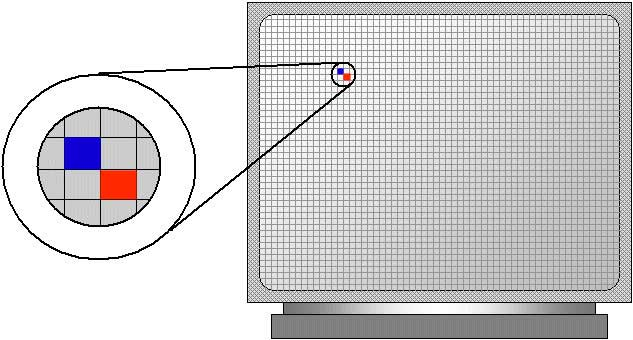
\includegraphics[scale=0.3]{Figures/pixel-definicion.jpg} 
	\caption{Representación gráfica de píxel\protect\footnotemark.}
	\label{fig:pixelimagen}
\end{figure}
\footnotetext{Imagen tomada de  \url{https://www.cavsi.com/preguntasrespuestas/images/pixel-definicion.jpg}}
%/http://aulainformatica.eu/datos/dise%C3%B1o_grafico/gimp/capitulo2/Teoria2.pdf

\subsection{Pitch}
Se define píxel pitch a la distancia física que separa a los leds que conforman la pantalla, esta distancia es medida en milímetros. La resolución de la pantalla tiene relación directa con el pitch, mientras más pequeño sea el pitch mayor será la resolución y viceversa\citep{IMAGENDEF2}. La figura \ref{fig:pixelpitch} muestra paneles led en los que se resalta el pitch.

Se suele abreviar esta medida con un "P-" seguida de la medida en milímetros. Por ejemplo la pantalla de esta memoria es una pantalla P-20.

\begin{figure}[htpb]
	\centering
	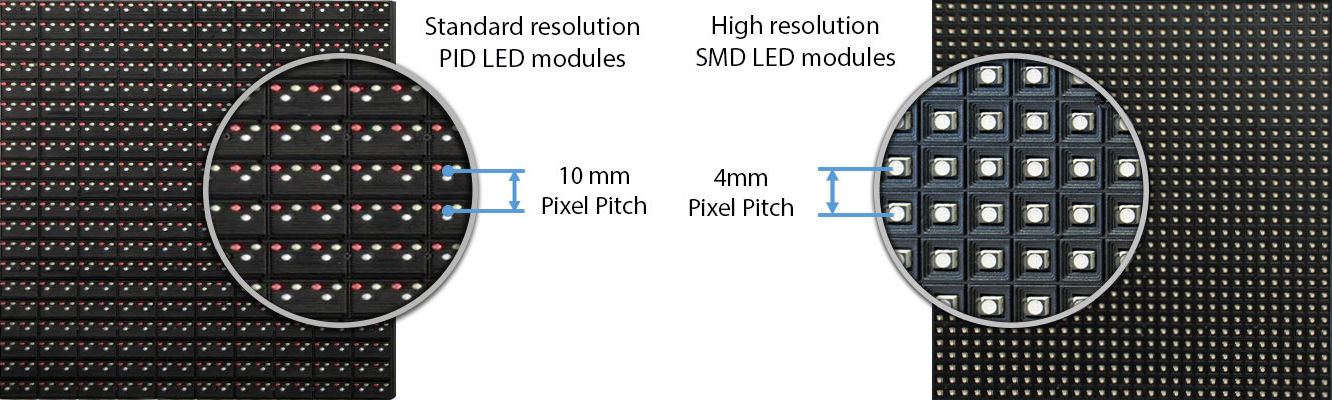
\includegraphics[scale=0.3]{Figures/pitch.jpg} 
	\caption{Representación gráfica de pitch\protect\footnotemark.}
	\label{fig:pixelpitch}
\end{figure}
\footnotetext{Imagen tomada de \url{https://www.finepixelled.com/theme/basic-knowledge/pixel-pitch-resolution.jpg}}



%/https://visualled.com/glosario/pixel-pitch/

\subsection{Resolución de pantalla}
La resolución de una pantalla se define como la cantidad de pixeles que esta posee.Se calcula multiplicando la cantidad de filas por el número de columnas\citep{WIKIRESOL}. La cantidad de detalles apreciable en la imagen tiene relación directa con la resolución, mientras mayor sea la resolución mayor cantidad de detalles se podrán apreciar en al imagen como se muestra en la figura \ref{fig:grafresolucion}.
\begin{figure}[htpb]
	\centering
	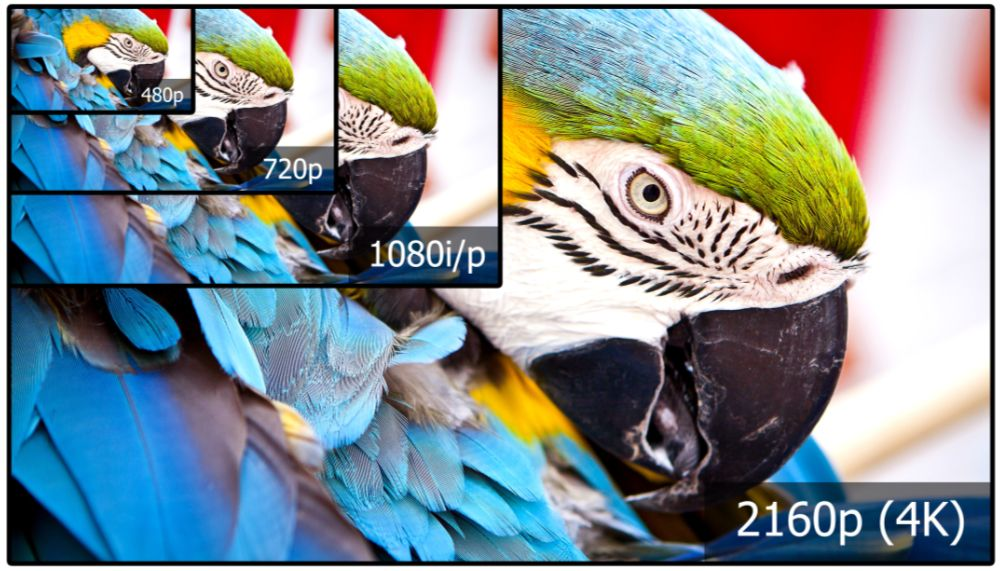
\includegraphics[scale=0.3]{Figures/resolucion.jpg} 
	\caption{Representación gráfica de resolución\protect\footnotemark.}
	\label{fig:grafresolucion}
\end{figure}
\footnotetext{Imagen tomada de \url{https://www.4kmonitor.net/wp-content/uploads/2020/03/4K-Monitor-Vor-und-Nachteile.jpg}}



\subsection{Representación de colores}
Para representar colores en pantallas se utiliza frecuentemente el modelo RGB en donde cada color es la suma de tres colores básicos rojo, verde y azul. La mezcla de estos tres colores con diferentes intensidades tratan de representar los colores una imagen real.
\begin{figure}[htpb]
	\centering
	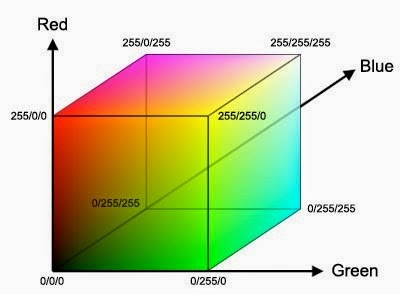
\includegraphics[scale=0.6]{Figures/modelorgb.jpg} 
	\caption{Modelo RGB\protect\footnotemark.}
	\label{fig:grafrgb}
\end{figure}
\footnotetext{Imagen tomada de \url{http://3.bp.blogspot.com/-NiYCndNGwHk/VCT\_ ywjC8FI/AAAAAAAAApk/0WDDtMziu6I/s1600/RGB1.jpg}}

\subsection{Tasa de refresco}
"La tasa de refresco es una magnitud que define la frecuencia con la que una pantalla actualiza el número de imágenes que muestra por segundo. Su principal diferencia con respecto al número de fotogramas por segundo está en que la frecuencia de refresco incluye el número de fotogramas idénticos que se reimprimen en la pantalla cada segundo, mientras que la segunda descarta estos en su medición. Su unidad de medida en el sistema internacional, al tratarse de una frecuencia, es el Hercio Hz" \citep{WIKITASA}.




\section{Paneles informativos comerciales}
Existen una gran cantidad de fabricantes de pantallas led P-20 para exteriores, el país líder en producción de pantallas led para exteriores es China. En la siguiente tabla\ref{tab:comercial} se muestra una comparación de las características de algunas pantallas comerciales.



\begin{table}[]
\caption[Pantallas comerciales]{Comparación de soluciones similares en el mercado.}
\begin{tabular}{|c|c|c|c|}
\textbf{Característica} & \textbf{Shenzhen Chuangkaiguang Co \citep{TABLAREF1}} & \textbf{Leeman \citep{TABLAREF2}} & \textbf{Samsung \citep{TABLAREF3}} \\
Angulo de visión        & H120,V60                             & H 120,V 60      & H140,V 59        \\
Constitución de pixel   & RGB                                  & RGB             & RGB              \\
Tasa de refresco        & mayor a 60hz                         & 60hz            & 60hz             \\
Consumo promedio        & 200w x m2                            & 200w x m2       & 169 w x m2       \\
Grado de protección     & IP65                                 & IP65            & IP65            
\end{tabular}
\label{tab:comercial}
\end{table}





\section{Propósito del proyecto}
El propósito de este proyecto es desarrollar una pantalla gigante full color led. Se espera que el desarrollo de este nuevo producto diversifique el portafolio de productos viales que ya posee la empresa.
\section{Alcance del proyecto}
El presente proyecto incluye:

\begin{itemize}
\item Desarrollo de prototipo usando la board DE1-SOC.
\item Desarrollo de hardware para control.
\item Desarrollo de hardware matrices de leds.
\item Desarrollo de firmware usando linux embebido.
\item Desarrollo de una GPU que maneje las matrices de leds con FPGA.
%\footnotetext{Referencia de placa  https://www.terasic.com.tw/cgi-bin/page/archive.pl?Language=English\&No=836}


\end{itemize}

El presente proyecto no incluye:

 \begin{itemize}
\item La interfaz gráfica para el cargado remoto de la imágenes.
\item La aplicación para cargar imágenes local.
\item Diseño de ventilación o mecánica de armado.

\end{itemize}




